\documentclass[UTF8]{article}
\usepackage{xcolor}
\usepackage{amsmath}
\usepackage{amssymb}
\usepackage{graphicx}
\usepackage{epstopdf}
\usepackage{inputenc}
\usepackage{geometry}
\geometry{left=2.5cm,right=2.5cm,top=2.5cm,bottom=2.5cm}

% For adding figures
\usepackage{graphicx}
\graphicspath{{./img/}}



\begin{document}

\title{
  NavyRecordReview \\
  \large A Performance Summary Report Visualization Tool
}

\author{CDR Tom Gardner and CDR Chase Gruszewski}
\date{15 March 2024}
\maketitle


\begin{abstract}
NavyRecordReview (NRR) is a data visualization tool to streamline the process of
drawing insights from a Naval Officer's Performance Summary Record (PSR). It 
automatically converts the PSR's dense, tabular text into a rich, intuitive, 
and interactive display \textcolor{red}{"dashboard"?}. All end-users of the PSR
can benefit from NavyRecordReview's functionality, from an individual Officer 
preparing their Letter-to-the-Board, to mentors conducting record reviews, to
Board Members preparing a record for briefing in "the tank." 
\end{abstract}



\begin{figure}[h!]
 \centering
 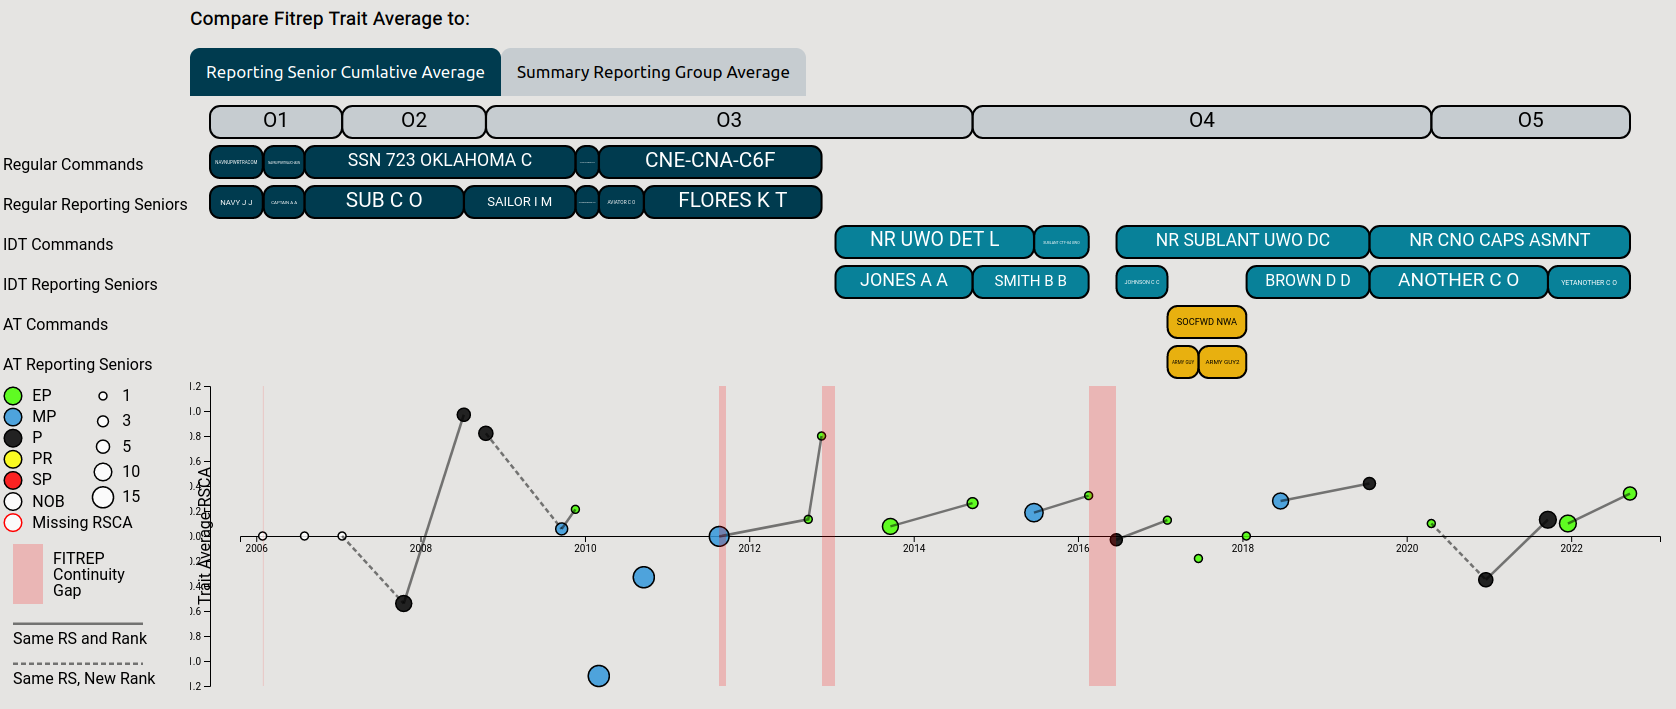
\includegraphics[width=0.75\textwidth]{nrr_dashboard.png}
 \caption{Sample NavyRecordReview PSR Visualization}
\end{figure}


\section{Background}
NavyRecordReview was born in March 2021 while Tom was serving as an Assistant
Recorder for the Fiscal Year 2022 FTS/RES O-6/O-5/O-4 CONT URL Selection Boards.
Due to the ongoing Covid-19 pandemic, these Boards were consolidated and
conducted by a single group of Recorders and Members. Consequently, Tom spent an
entire month at the Bureau of Naval Personnel, much of which was spent
observing Members review and brief PSRs. This process struck Tom as wildly
inefficient, sometimes ineffective, and in all cases, ripe for improvement.\\

For anyone who participates in a promotion Board, it quickly becomes apparent
that the goal of a Board Member's record review is to gain an understanding of
an Eligible's demonstrated performance and convey that understanding to the
other Board Members. This understanding comes not from personal knowledge of
Eligible, but from reviewing documents in their official record - primarily the
PSR and Fitness Reports (FITREPs).\\

%The PSR (figure 2) is a table of column and rows of data summarizing all of the
%FITREPs an officer has recieved over the course of their career. 

Board Members perform tasks during record review that we categorize into two
types:
\textit{\textbf{rote}} and \textit{\textbf{expert}}. Examples of each follow:\\

\textit{\textbf{Rote}} tasks: 
\begin{itemize}
  \item Checking each FITREP for continuity with the previous FITREP.
  \item Comparing each FITREP Trait Average to the Reporting Senior's Cumulative
  Average (RSCA).
  \item Checking for Promotion Recommendations that "break right."
  \item Checking for increasing Trait Averages among successive FITREPs from the
  same Reporting Senior. 
\end{itemize}

\textit{\textbf{Expert}} tasks: 
\begin{itemize}
  \item Evaluating career progression through demonstrated performance in
  demanding positions.
  \item Evaluating the comments in Block 41 of FITREPs to gain insight into 
  performance during specific periods of an Eligible's career
  \item Deciding what elements of the applicable Community Brief the Eligible
  has satisfied and whether there may be any amplifying information for
  shortcomings.
\end{itemize}

\begin{figure}[h!]
 \centering
 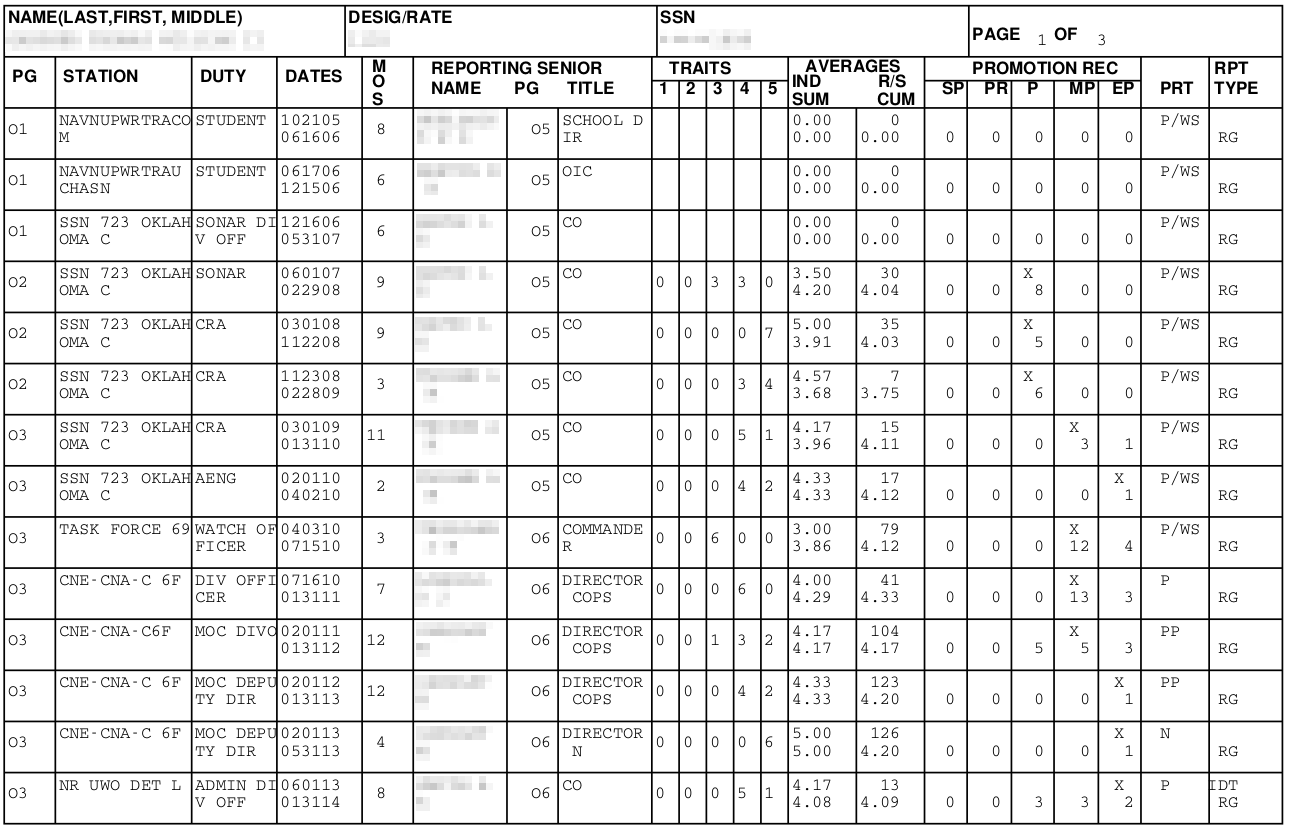
\includegraphics[width=0.95\textwidth]{blurred_psr.png}
 \caption{Sample PSR (redacted)}
\end{figure}

Doing that by looking at a rectangular table of data, doing some "arts and crafts" on it, and showing them the marked up rectangle of data is neither efficient nor effective. What they needed was an automated, consistent, and intuitive way to visualize the data contained in a PSR.

I saw first hand that Board Members marked up PSRs differently from each other, causing the other Members to have to mentally switch each time a different Member stood up to brief a record, remembering things like how that particular Member annotates FITREP trait averages with respect to RSCA (e.g., does this guy draw an arrow high-to-low, an arrow low-to-high, circle the higher number, or circle the lower number). I saw many times that a Member's annotations were wrong (e.g., they said a FITREP trait average was below RSCA when it wasn't). I watched as Members painstakingly looked for FITREP continuity gaps, mind-numbingly comparing thousands of dates, written on different lines in MMDDYY format, to each other to to see if there are any days in between, trying to keep straight how many days are in a given month, what years are leap-years, etc. Let's just say, "mistakes were made," and it took days or weeks longer than it should have.

I worked on a prototype to demonstrate the idea. I cornered anyone I could, trying to sell them on my idea. I talked with NPC Staff, Board Members, my Board President. Some of them had a lot of Board experience and seemed resistant to any change. Some people though it made sense in principal, but wouldn't work on a real PSR, so I hand-drew the visualization of my personal PSR, which is attached. RADM (ret) Lennon was in the building as a Member on a different Boards, and I knew he would be interested, so I took an opportunity to present my idea to him in the break room. He was the first person who, rather than saying, "That's a great idea," and handing my prototype back to me said, "That's a great idea, can I have this?" He shared the idea with VADM Mustin, who was also present for a Board. VADM Mustin liked the idea and, I believe, encouraged RADM Lennon to champion it in his capacity as Vice Director of the Naval Staff.

Seeing that the idea was gaining traction at the highest levels of the Navy, I got to work further implementing (programming) the idea. Eventually I was able to recruit Chase, an extremely skilled web developer, to work on the idea with me. We setup some infrastructure for version control and deployment of our code and bought a domain. We have continued to develop the project, which is what you see at www.navyrecordreview.com.

\section{Functionality}
\begin{itemize}
  \item \textbf{Automated Parsing} The system will automatically build a reporting by scanning a PSR PDF. While it says "upload," this is a bit of a misnomer, as nothing is ever sent to our servers and all code runs inside the user's browser (ie "client-side" processing).
  \item \textbf{Trait Average Comparision} The system allows comparison of the individuals trait average to the reporting senior cumulative average (RCSA) or the summary group average, creating a contextual view of the individual's performance.
  \item \textbf{Performance Trend Lines} Evaluations by the same reporting senior, at the same command are connected by solid trend lines showing if performance has trended upward or downwards.
  \item \textbf{FITREP Gap Identification} Gaps in an indiviuals record are highlighted in red, quickly identifying any periods of time that might need to be addressed.
  \item \textbf{Manual Entry and Editing} Records can be completely manually entered as well. The PSR table allows manual entry of performance data. Additionally, this table can be used to correct errors in the PSR, such as misspellings in the Command Name (discussed further in the Goals and Backlog section).
  \item \textbf{Date Range Selection} It's rare to need to review an individuals entire record, so the "Start Date" selector allows reviewers to zoom in on a specified period of time so the individuals most recent performance trends are clearer.
  \item \textbf{Multiple FITREP Comparison} One of our newer features, this allows multiple PSRs to be enetered at once. Reviewers can quickly toggle between PSRs by selecting the individuals name, or view multiple records side by side. In Multiview, records can either be compared across the past 2 paygrades, or the past 5 years.
\end{itemize}

\section{Use Cases}
Presently, the NavyRecordReview PSR Visualization project envisions 3 distinct use cases:
\begin{enumerate}
\item \textbf{Board Reviews} The insipiration, and primary purpose for the project is to provide a better way to visualize the trait avergae performance and promotion recommendations for an individual service member and assist with assessing their historic level of performance. To be clear, this system is not intended to replace the need for the human review of an individual service record during a board. It is intended to provide a clear assessment of the discrete numerical information in a performance record including promotion recommendations, trait averages vs. reporting senior cumulative averages, trait averages vs summary group averages, and performance trends across reporting seniors and commands. This should free board members' time in processing records to spend less time comparing numbers on a PSR, and more time for reviewing the context (e.g. Block 41 information), of the service member's performance.
\item \textbf{Reporting Senior Assessments} By their very nature, FITREPs are comparative evaluations, with the burdern of assessing which individuals are most suitable for promtion falling to the reporting senior. In assessing each summary groups rankings, reporting seniors no only assess performance for the period of report, but also the overall suitablility of the individual for promotion which may include additional factors such as time in grade, history of performance, history of assignments, additional qualification, and others. To provide reporting seniors with and additional tool to assess these additional factors, the NavyRecordReview PSR project provides the option to upload multiple PSRs from individuals, and see them compared side by side, saving time and providing a graphical representation of these additional factors that may assist in ranking personnel within a summary group.
\item \textbf{Individual Record Reviews} By extension of use cases 1 and 2, the ability for individuals and the mentors to get a quick snapshot of the career performance is valuable when preparing for boards, or mapping out the next waypoints in their career. The PSR visualization project provides the opportunty for the boards, reporting seniors, and individual to all share the same graphical view of the individual's performance throughout their career.
\end{enumerate}


\section{Goals and Backlog}
In our efforts to continuously improve the NavyRecordReview PSR Visualization project, we've worked with fellow sailors, human resource experts, flag officers, and BUPERS staff. Some of the main items in our current goals list include:
\begin{itemize}
    \item \textbf{Improved Aesthetics} Presently, the project operates on a functional, no frills design. While useable, it is not particularly delightful to use. We intend to improve the appearance of the project by enhancing the table (below the graph) to match the PSR PDF that is generated by BUPERS, and simplify the process for making edits. Additionally, we intend to expand the FAQ section and instructional information to offer users resources to help understand how they can assess PSRs using the tool. In our more ambitious moments, we'd like to run user testing with a cohort of ~10 x O-6s to see how they interact with the system and what UI/UX changes could be made to improve the experience for this user group.

    \item \textbf{Data Smoothing} In the development of this project, we've found that it's very common for an individual's PSR to contain minor variances from year to year that can confuse the graphical representation of the data. Generally these include minor variances in the spelling/ abbreviation of a command name, primary duty, or reporting senior title. Presently, these mistakes can be corrected using the program's manual editting feature to manual smooth the data. This works, but can be time consuming. To help improve the user experience, we intend to offer automated data smoothing, where the program will look for spellings that are very close together and offer a "did you me" suggestion for making them the same.

    \item \textbf{Expand Applicability} 

    \item \textbf{Direct PSR parsing} Currently, the program builds a PSR assessment by scanning PSR pdf and looking for information at specific coordinates on the PDF. To date, this has worked reliably, but it is a "brittle" solution -- meaning that a small change in the way the PSR PDF's are styled/ generated, and the whole system might break and require an update. Ideally, we'd want the PSR visualization system to be integrated into BOL's suite of tools, where it could directly pull data points from the individual's record and use the information to populate the graph. This goal depends on adoption by the Navy and partnership with BUPERS to implement the system.

\end{itemize}

\section{Past Efforts at Fostering Adoption/Briefing Record/Praise for NavyRecordReview}


%\subsection{Sub Section}

CDR Chase Gruszewski and I maintain NavyRecordReview.com. We are both SELRES with NR CNO Capabilities and Assessments, N81R.

The idea came from my experience as an Assistant Recorder for the FY-22 FTS/RES O-6/O-5/O-4 CONT URL Selection Boards. That was during the peak of Covid, so they consolidated those Boards somewhat, having a single group of Members and Recorders execute all 5 Boards. I spent the entire month of March 2021 in Millington and much of that time was spent watching Members markup PSRs in, as I saw it, a very inefficient manner. I'm a programmer and I do a lot of data science/data analytics. As much as anything else in data science, I really enjoy data visualization. It was obvious to me that the task of record review by a Board Member is to gain an understanding of an Eligible's past performance and convey that understand to the other Board Members. Doing that by looking at a rectangular table of data, doing some "arts and crafts" on it, and showing them the marked up rectangle of data is neither efficient nor effective. What they needed was an automated, consistent, and intuitive way to visualize the data contained in a PSR.

I saw first hand that Board Members marked up PSRs differently from each other, causing the other Members to have to mentally switch each time a different Member stood up to brief a record, remembering things like how that particular Member annotates FITREP trait averages with respect to RSCA (e.g., does this guy draw an arrow high-to-low, an arrow low-to-high, circle the higher number, or circle the lower number). I saw many times that a Member's annotations were wrong (e.g., they said a FITREP trait average was below RSCA when it wasn't). I watched as Members painstakingly looked for FITREP continuity gaps, mind-numbingly comparing thousands of dates, written on different lines in MMDDYY format, to each other to to see if there are any days in between, trying to keep straight how many days are in a given month, what years are leap-years, etc. Let's just say, "mistakes were made," and it took days or weeks longer than it should have.

I worked on a prototype to demonstrate the idea. I cornered anyone I could, trying to sell them on my idea. I talked with NPC Staff, Board Members, my Board President. Some of them had a lot of Board experience and seemed resistant to any change. Some people though it made sense in principal, but wouldn't work on a real PSR, so I hand-drew the visualization of my personal PSR, which is attached. RADM (ret) Lennon was in the building as a Member on a different Boards, and I knew he would be interested, so I took an opportunity to present my idea to him in the break room. He was the first person who, rather than saying, "That's a great idea," and handing my prototype back to me said, "That's a great idea, can I have this?" He shared the idea with VADM Mustin, who was also present for a Board. VADM Mustin liked the idea and, I believe, encouraged RADM Lennon to champion it in his capacity as Vice Director of the Naval Staff.

Seeing that the idea was gaining traction at the highest levels of the Navy, I got to work further implementing (programming) the idea. Eventually I was able to recruit Chase, an extremely skilled web developer, to work on the idea with me. We setup some infrastructure for version control and deployment of our code and bought a domain. We have continued to develop the project, which is what you see at www.navyrecordreview.com.

On April 26, 2021, RADM Lennon sent an email to Chief of Naval Personnel, ADM Nowell, Commander, Navy Personnel Command, RADM Hosley, Chief of Naval Reserve, VADM Mustin, SES Mark Livingston, and SES Patrick Barrett describing the idea and attaching a scanned copy of the original prototype. CNP liked the idea and directed RADM Holsey to include me as a part of the virtual team working Board process improvements (excerpts from the exchange below, for context). They eventually got me linked up with Steven Skretkowicz and Martin Pompeo at NPC. We had a good exchange going, in which we discussed their requirements, my rationale behind the idea, the application of different principles of data visualization to the PSR, etc. After 4 to 5 emails back-and-forth, I stopped receiving replies from these gentlemen.

Other attempts to gain traction have included discussing with CAPT Peppel, the CNRF CIO, who sent an email on 01 Sep 2021 to CAPT Eric Johnson and Mr. Jay Steffenhagen, with no response. For a time, I was going through my then-employer, Metron Scientific Solutions, Inc., to consider a business development opportunity to get NPC commercially interested. Many members of my unit have shared the idea with "people in high places" that they know - most of whom think it's a great idea and that's as far as it goes. We entered the i3 Waypoints contest, but the only feedback from that process was that we were not selected as a finalist.

That is the short history of the project. I know implementing this sort of thing can take a very long time, so I've tried not to expect too much change too quickly. However, seeing leads fizzle out has been pretty disheartening at times. I do all of the work on NRR in my free time, so there are times when I spend a lot effort improving it and other long stretches when it sits dormant. Sometimes I think the Navy would be more interested if I were Booz Allen Hamilton trying to sell it to them for \$5 million than if I am a Reservist trying to give it to them for free. Chase and I have considered everything from forming an LLC to try to sell this idea to the Navy to asking Kelly Beamsley to put the link on his website and never working on the code again.

If you have any interest, I'd be more than happy to discuss anything about the project with you.


\end{document}


